%%%%%%%%%%%%%%%%%%%%%%%%%%%%%%%%%%%%%%%%%
% Beamer Presentation
% LaTeX Template
% Version 1.0 (10/11/12)
%
% This template has been downloaded from:
% http://www.LaTeXTemplates.com
%
% License:
% CC BY-NC-SA 3.0 (http://creativecommons.org/licenses/by-nc-sa/3.0/)
%
%%%%%%%%%%%%%%%%%%%%%%%%%%%%%%%%%%%%%%%%%

%----------------------------------------------------------------------------------------
%	PACKAGES AND THEMES
%----------------------------------------------------------------------------------------

\documentclass{beamer}

\mode<presentation> {

% The Beamer class comes with a number of default slide themes
% which change the colors and layouts of slides. Below this is a list
% of all the themes, uncomment each in turn to see what they look like.

%\usetheme{default}
%\usetheme{AnnArbor}
%\usetheme{Antibes}
%\usetheme{Bergen}
%\usetheme{Berkeley}
\usetheme{Berlin}
%\usetheme{Boadilla}
%\usetheme{CambridgeUS}
%\usetheme{Copenhagen}
%\usetheme{Darmstadt}
%\usetheme{Dresden}
%\usetheme{Frankfurt}
%\usetheme{Goettingen}
%\usetheme{Hannover}
%\usetheme{Ilmenau}
%\usetheme{JuanLesPins}
%\usetheme{Luebeck}
%\usetheme{Madrid}
%\usetheme{Malmoe}
%\usetheme{Marburg}
%\usetheme{Montpellier}
%\usetheme{PaloAlto}
%\usetheme{Pittsburgh}
%\usetheme{Rochester}
%\usetheme{Singapore}
%\usetheme{Szeged}
%\usetheme{Warsaw}

% As well as themes, the Beamer class has a number of color themes
% for any slide theme. Uncomment each of these in turn to see how it
% changes the colors of your current slide theme.

%\usecolortheme{albatross}
%\usecolortheme{beaver}
%\usecolortheme{beetle}
%\usecolortheme{crane}
%\usecolortheme{dolphin}
%\usecolortheme{dove}
%\usecolortheme{fly}
%\usecolortheme{lily}
%\usecolortheme{orchid}
%\usecolortheme{rose}
%\usecolortheme{seagull}
%\usecolortheme{seahorse}
%\usecolortheme{whale}
%\usecolortheme{wolverine}

%\setbeamertemplate{footline} % To remove the footer line in all slides uncomment this line
%\setbeamertemplate{footline}[page number] % To replace the footer line in all slides with a simple slide count uncomment this line

%\setbeamertemplate{navigation symbols}{} % To remove the navigation symbols from the bottom of all slides uncomment this line
}

\usepackage{graphicx} % Allows including images
\usepackage{booktabs} % Allows the use of \toprule, \midrule and \bottomrule in tables
%\usepackage[brazilian]{babel}
\usepackage[utf8]{inputenc}
\usepackage{listings}
\usepackage{amsmath}
\usepackage{amsfonts}
\usepackage{pdfpages}
\usepackage{textpos}

\graphicspath{ {img/} }

%----------------------------------------------------------------------------------------
%	TITLE PAGE
%----------------------------------------------------------------------------------------

\title[Generating Acrostics via Paraphrasing and Heuristic Search]{Generating Acrostics via Paraphrasing and Heuristic Search} % The short title appears at the bottom of every slide, the full title is only on the title page

\author[Bruno, Fernando, Jürgen, William]{Bruno Soares Fillmann\\
Fernando Bombardelli da Silva\\
Jürgen Bauer\\
William Bombardelli da Silva
} % Your name
\institute[TU Berlin] % Your institution as it will appear on the bottom of every slide, may be shorthand to save space
{
Technische Universität Berlin \\ % Your institution for the title page
Datenbanksysteme und Informationsmanagement \\
DBPRO – Database Projects (WS 2014/2015) \\
\medskip
%\textit{fbdasilva@inf.ufrgs.br} % Your email address
}
\date{12.01.2015} % Date, can be changed to a custom date

\begin{document}

\begin{frame}
\titlepage % Print the title page as the first slide
\end{frame}

\begin{frame}
\frametitle{Organization} % Table of contents slide, comment this block out to remove it
\tableofcontents % Throughout your presentation, if you choose to use \section{} and \subsection{} commands, these will automatically be printed on this slide as an overview of your presentation
\end{frame}

%----------------------------------------------------------------------------------------
%	PRESENTATION SLIDES
%----------------------------------------------------------------------------------------

%------------------------------------------------
\section{Overview} % Sections can be created in order to organize your presentation into discrete blocks, all sections and subsections are automatically printed in the table of contents as an overview of the talk
%------------------------------------------------

%\subsection{Subsection Example} % A subsection can be created just before a set of slides with a common theme to further break down your presentation into chunks

\begin{frame}
\frametitle{The Problem}
\begin{itemize}
\item Given a text T and an acrostic X, find a paraphrased version of T that encodes X in the first letters of each line.
\end{itemize}

\texttt{\tiny Knuth ist der Sohn eines Lehrers. Er besuchte die Milwaukee Lutheran \\
High School und begann sein Physikstudium am California Institute of \\
Technology im September 1956. Aus zweierlei Gründen schlug er \\
tatsächlich seinem zweiten Studienjahr jedoch den Weg zur Mathematik \\
ein: Zum einen löste er ein Problem eines seiner \\
Mathematikprofessoren, was ihm eine 1,0 als Note einbrachte, zum \\
anderen fand er wenig Gefallen an den physikalischen Praktika. Er \\
erhielt einen Bachelor- und einen Master-Abschluss 1960 an der Case \\
Western Reserve University. \\}

Result Text: \\

\texttt{\scriptsize{K}\tiny nuth ist der Sohn eines Lehrers. Er besuchte die Milwaukee Luthera- \hskip 18pt \emph{//Wrong Hyphenation} \\
\scriptsize{n} \tiny  High School und begann sein Physikstudium am California Instit- \hskip 33pt \emph{//Line Break +} \\
\scriptsize{u}\tiny te of Technology im September 1956. Aus zweierlei Gründen schlug er \hskip 23pt \emph{//Wrong Hyphenation} \\
\scriptsize{t}\tiny atsächlich seinem zweiten Studienjahr jedoch den Weg zur Mat- \hskip 39pt \emph{//Wrong Hyphenation} \\
\scriptsize{h}\tiny ematik ein: Zum einen löste er ein Problem eines seiner \\
Mathematikprofessoren, was ihm eine 1,0 als Note einbrachte, zum \\
anderen fand er wenig Gefallen an den physikalischen Praktika. Er \\
erhielt einen Bachelor- und einen Master-Abschluss 1960 an der Case \\
Western Reserve University. \\}
\end{frame}


\begin{frame}
\frametitle{The Project}
\begin{itemize}
\item \textbf{Main goal of the project:} Implement the paper for the German language.
\item \textbf{Main idea of the algorithm:}
	\begin{itemize}
	\item Modeled as a search problem in a tree.
	\item The vertices are states (texts) and the edges are operations over states.
	\item Artificial intelligence is applied for the search strategy (A* Algorithm).
	\end{itemize}
\end{itemize}
\end{frame}

\begin{frame}
\frametitle{Last State of Work}
\begin{itemize}
\item Line Break and Wrong Hyphenation working properly
\item Search algorithm working properly
\item Word Insertion working partially, but Deletion not working
\end{itemize}
\end{frame}

%------------------------------------------------
\section{New Operations}
%------------------------------------------------
\begin{frame}
\frametitle{New Developed Operations}
\begin{itemize}
	\item Word Insertion Or Deletion (Enhancements)
	\item Synonym
	\item Hyphenation
	\item Spelling
\end{itemize}
\end{frame}

%************** SYNONYM START *******************
\begin{frame}
\frametitle{Synonym}
\begin{itemize}
	\item Free dictionary of synonyms is used, namely, Open Thesaurus (www.openthesaurus.de)
	\item We use \textbf{Redis} as database server (NoSQL)
	\item Redis stores data as key-value pairs
	\item Our base is structured in a way that, every word in the thesaurus is a key that points to a set of synonyms
	\item The thesaurus text file is imported into the database by a Python script
	\item The database is then consulted by the application during its execution
\end{itemize}
\end{frame}
%************** SYNONYM END *******************

%***********HYPHENATION START *******************************************
%This is the 1st slide!!
\begin{frame}
\frametitle{Hyphenation}


\begin{itemize}
\item Line Length constraints $l_{min}=50$ and $l_{max}=70.$



\item For hyphenation a re-implementation of Knuth's hyphenation algorithm in
TeX is used (TEXHyphenator-J by David Tolpin) 

\item A word can be hyphenated if: The part of the current line \textbf{from} the beginning \textbf{to} the hyphen has a length of at least $l_{min}=50.$

\item The text \textbf{after} the hyphen has to be aligned again to fulfill the line length
constraints.



\item A greedy word wrap algorithm is applied. 

\item Don't allow words of length $>20$ in the start text.
\end{itemize}

\end{frame}


%This is the 2nd slide!!
\begin{frame}
\frametitle{Hyphenation}




\begin{itemize}


\item \textbf{Example:}
\item 38 hyphenations!


\end{itemize}

\begin{picture}(300,400)
\put(-10,-165){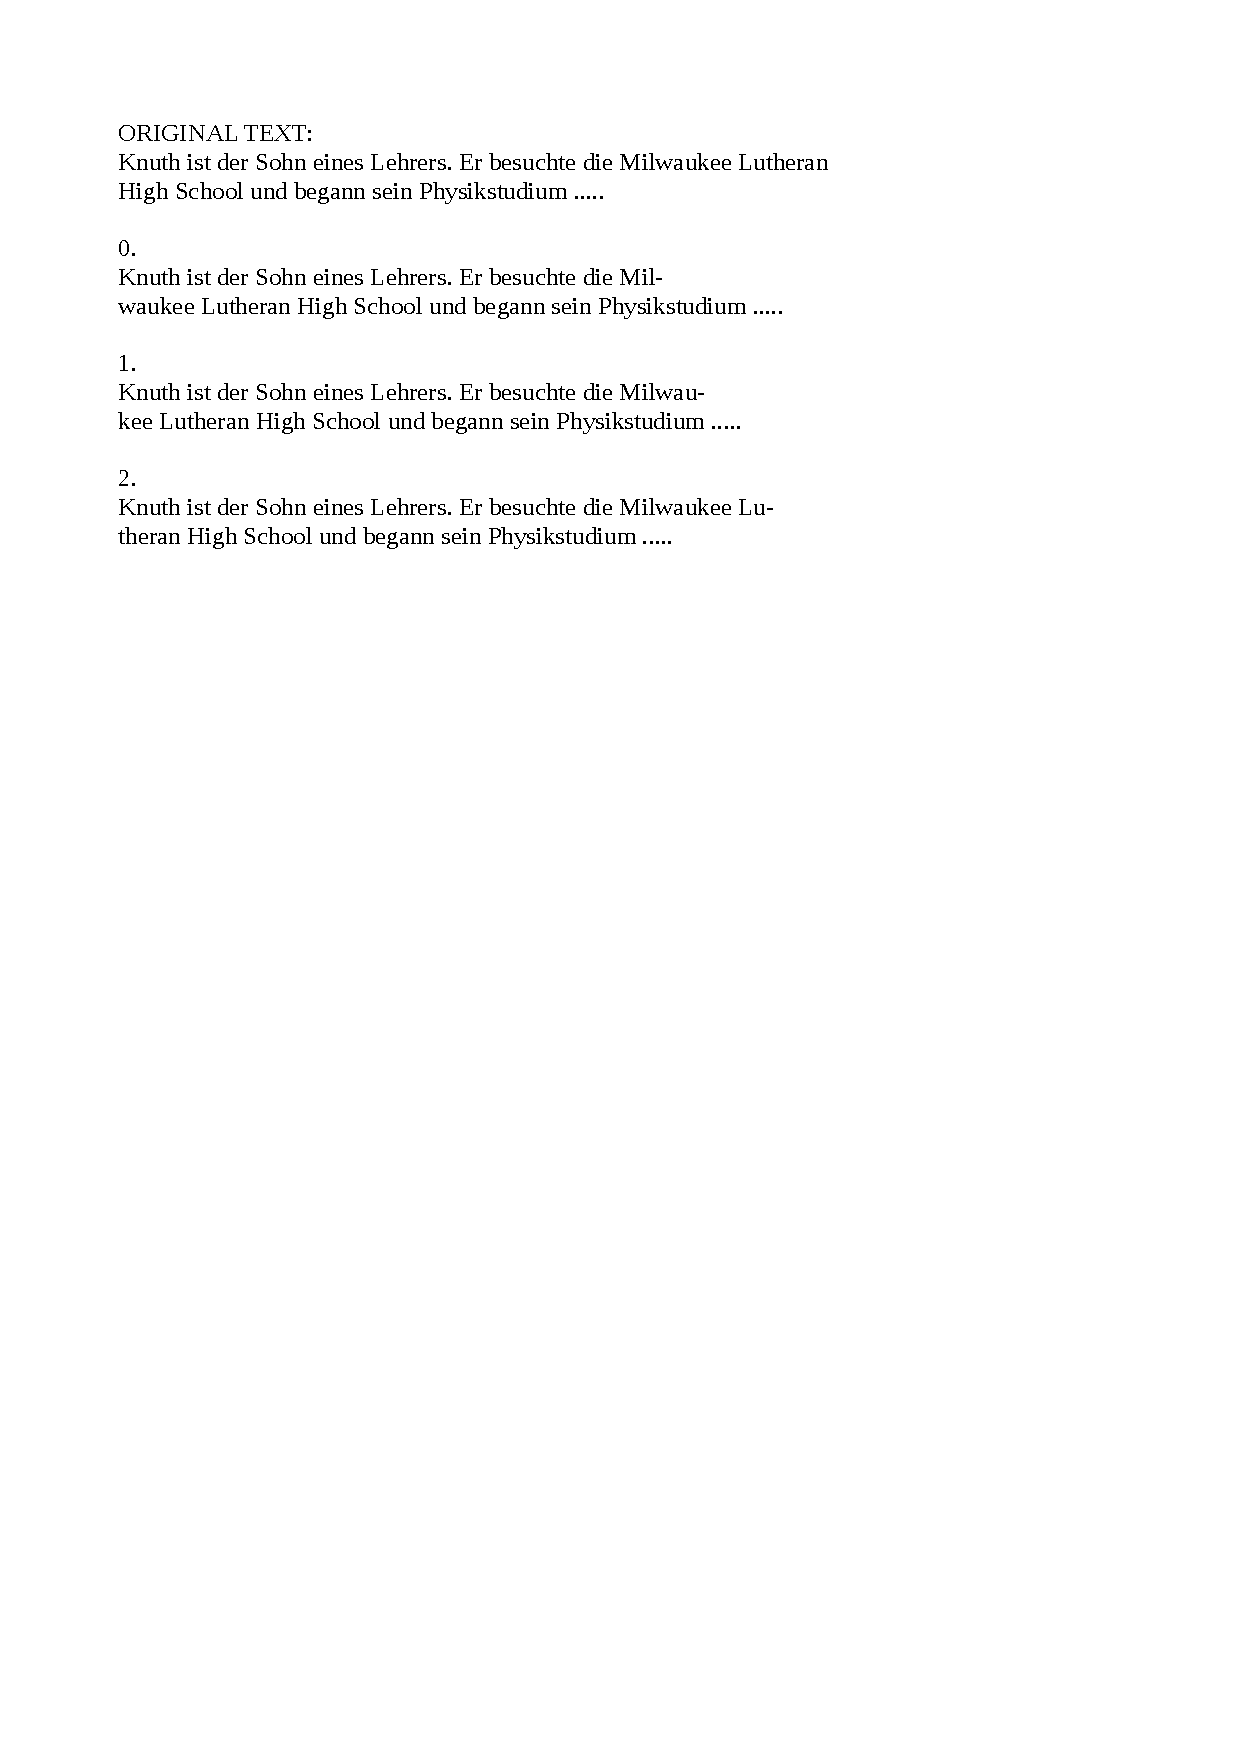
\includegraphics[scale=0.7]{KnuthHyphenation.pdf}}
\end{picture}



\end{frame}

%***********HYPHENATION END ****************************************************

%***********SPELLING START ****************************************************
\begin{frame}
\frametitle{Spelling}
\begin{itemize}
	\item This operation adds wrong spellings of words to add letter variety
	\item To do this it changes letters such as 'ä', 'ö' and 'ü' to respectively ae oe ue.
	\item The german letter 'ß' can also be changed to 'ss'
	\item Only one word is changed per new text created by this operation
\end{itemize}
\end{frame}

\begin{frame}
\frametitle{Results $-$ Spelling}

Original Text: \\

\texttt{\tiny Die etymologischen Vorformen von "deutsch" bedeuteten ursprünglich \\
"zum Volk gehörig", wobei das Adjektiv zunächst die Dialekte des \\
kontinental-westgermanischen Dialektkontinuums bezeichnete. Die \\
Bezeichnung Deutschland wird seit dem 15. Jahrhundert verwendet, ist \\
in einzelnen Schriftstücken aber schon früher bezeugt. \\}

Result Text: \\

\texttt{\tiny Die etymologischen Vorformen von "deutsch" bedeuteten urspru- \\
englich "zum Volk gehörig", wobei das Adjektiv zunächst die Dialekte de- \\
s kontinental-westgermanischen Dialektkontinuums bezeichnete. Die \\
Bezeichnung Deutschland wird seit dem 15. Jahrhundert verwendet, ist \\
in einzelnen Schriftstücken aber schon früher bezeugt. \\}
\end{frame}


%***********SPELLING END ****************************************************


%------------------------------------------------
\section{New Results}
%------------------------------------------------

%************** DELETION START *******************
\begin{frame}
\frametitle{Results $-$ Insertion Of New Words}
\texttt{\tiny
Im Englischen bedeutet blau sein so etwas wie traurig oder deprimiert \\
sein, weltbekannt ist die Musikrichtung Blues. Das ist traurig aber. Im \\
Deutschen hat blau sein allerdings eine ganz andere Bedeutung. Wenn \\
jemand eine feucht-fröhliche Party feiert (also eine, auf der viel \\
Alkohol getrunken wird), dann ist er hinterher wahrscheinlich blau. \\
Blau sein bedeutet im Deutschen nämlich betrunken sein. \\
}

Result Text: \\

\texttt{\scriptsize{I}\tiny m Englischen bedeutet blau sein so etwas wie traurig oder \hskip 58pt \emph{//Line Break} \\
\scriptsize{d}\tiny eprimiert sein, weltbekannt ist die Musikrichtung Blues. Das ist \\
\scriptsize{e}\tiny cht traurig aber. Im Deutschen hat blau sein allerdings \hskip 60pt \emph{//Word Insertion}\\
\scriptsize{e}\tiny ine ganz andere Bedeutung. Wenn jemand eine feucht-fröhliche Party \hskip 30pt \emph{//+ Line Break}\\
feiert (also eine, auf der viel Alkohol getrunken wird), dann ist er \\
hinterher wahrscheinlich blau. Blau sein bedeutet im Deutschen nämlich \\
betrunken sein. \\
}
\end{frame}

\begin{frame}
\frametitle{Results $-$ Deletion Of Words}
\texttt{\tiny
In diesen Auflagen könnte denn auch der Hebel liegen, um Griechenland \\
weiteres Geld zu verweigern. Denn ein Stopp der Zinszahlungen dürfte \\
als Verstoß gegen das Rettungsprogramm gewertet werden. Denn für alle \\
Geschäftbanken in der Eurozone gilt: Geld von der EZB gibt es nur \\
mäßig, wenn die Finanzinstitute eine bestimmte Menge an Wertpapieren, \\
zum Beispiel Staatsanleihen, als Pfand bei der EZB hinterlegen. In \\
diesem Fall könnte die EZB ihre Ansprüche an die Sicherheiten wieder \\
erhöhen. \\
}

Result Text: \\

\texttt{\scriptsize{I}\tiny n diesen Auflagen könnte denn auch der Hebel liegen, um Grieche-  \hskip 30pt \emph{//Wrong Hyphenation} \\
\scriptsize{n}\tiny land weiteres Geld zu verweigern. Denn ein Stopp der Zinszahlungen dürf- \emph{//Wrong Hyphenation} \\
\scriptsize{t}\tiny e als Verstoß gegen das Rettungsprogramm gewertet werden. Denn für alle \\
\scriptsize{i}\tiny n der Eurozone gilt: Geld von der EZB gibt es nur \hskip 72pt \emph{//Word Deletion} \\
\scriptsize{m}\tiny äßig, wenn die Finanzinstitute eine bestimmte Menge an Wertpapieren, \\
zum Beispiel Staatsanleihen, als Pfand bei der EZB hinterlegen. In \\
diesem Fall könnte die EZB ihre Ansprüche an die Sicherheiten wieder \\
erhöhen. \\
}
\end{frame}

%************** DELETION END *******************

%************** SYNONYM START *******************
\begin{frame}
\frametitle{Results $-$ Synonym}
\begin{figure}
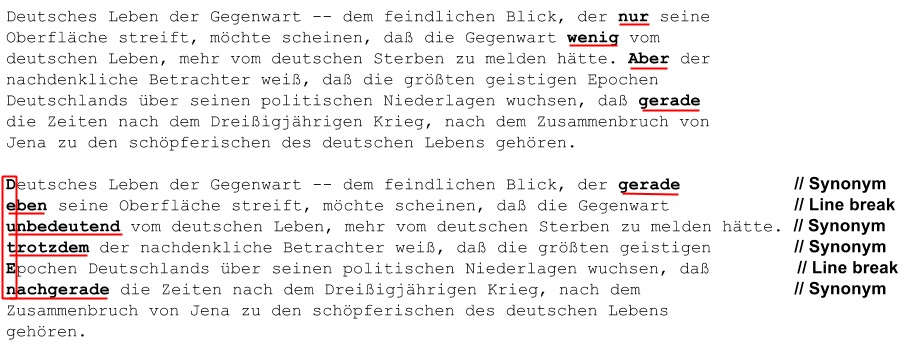
\includegraphics[scale=0.35]{beispiel-synonym}
\end{figure}
\end{frame}
%************** SYNONYM END *******************

%********************START GENERAL EXAMPLE (all Operators included)***************************************************

% 1st Slide
\begin{frame}
\frametitle{Results $-$ Hyphenation}


\begin{itemize}

\item  1 min 22 sec, 17517 nodes, Ops: Hyph,WrHyph,LB


\end{itemize}

\begin{picture}(300,400)
\put(-10,-165){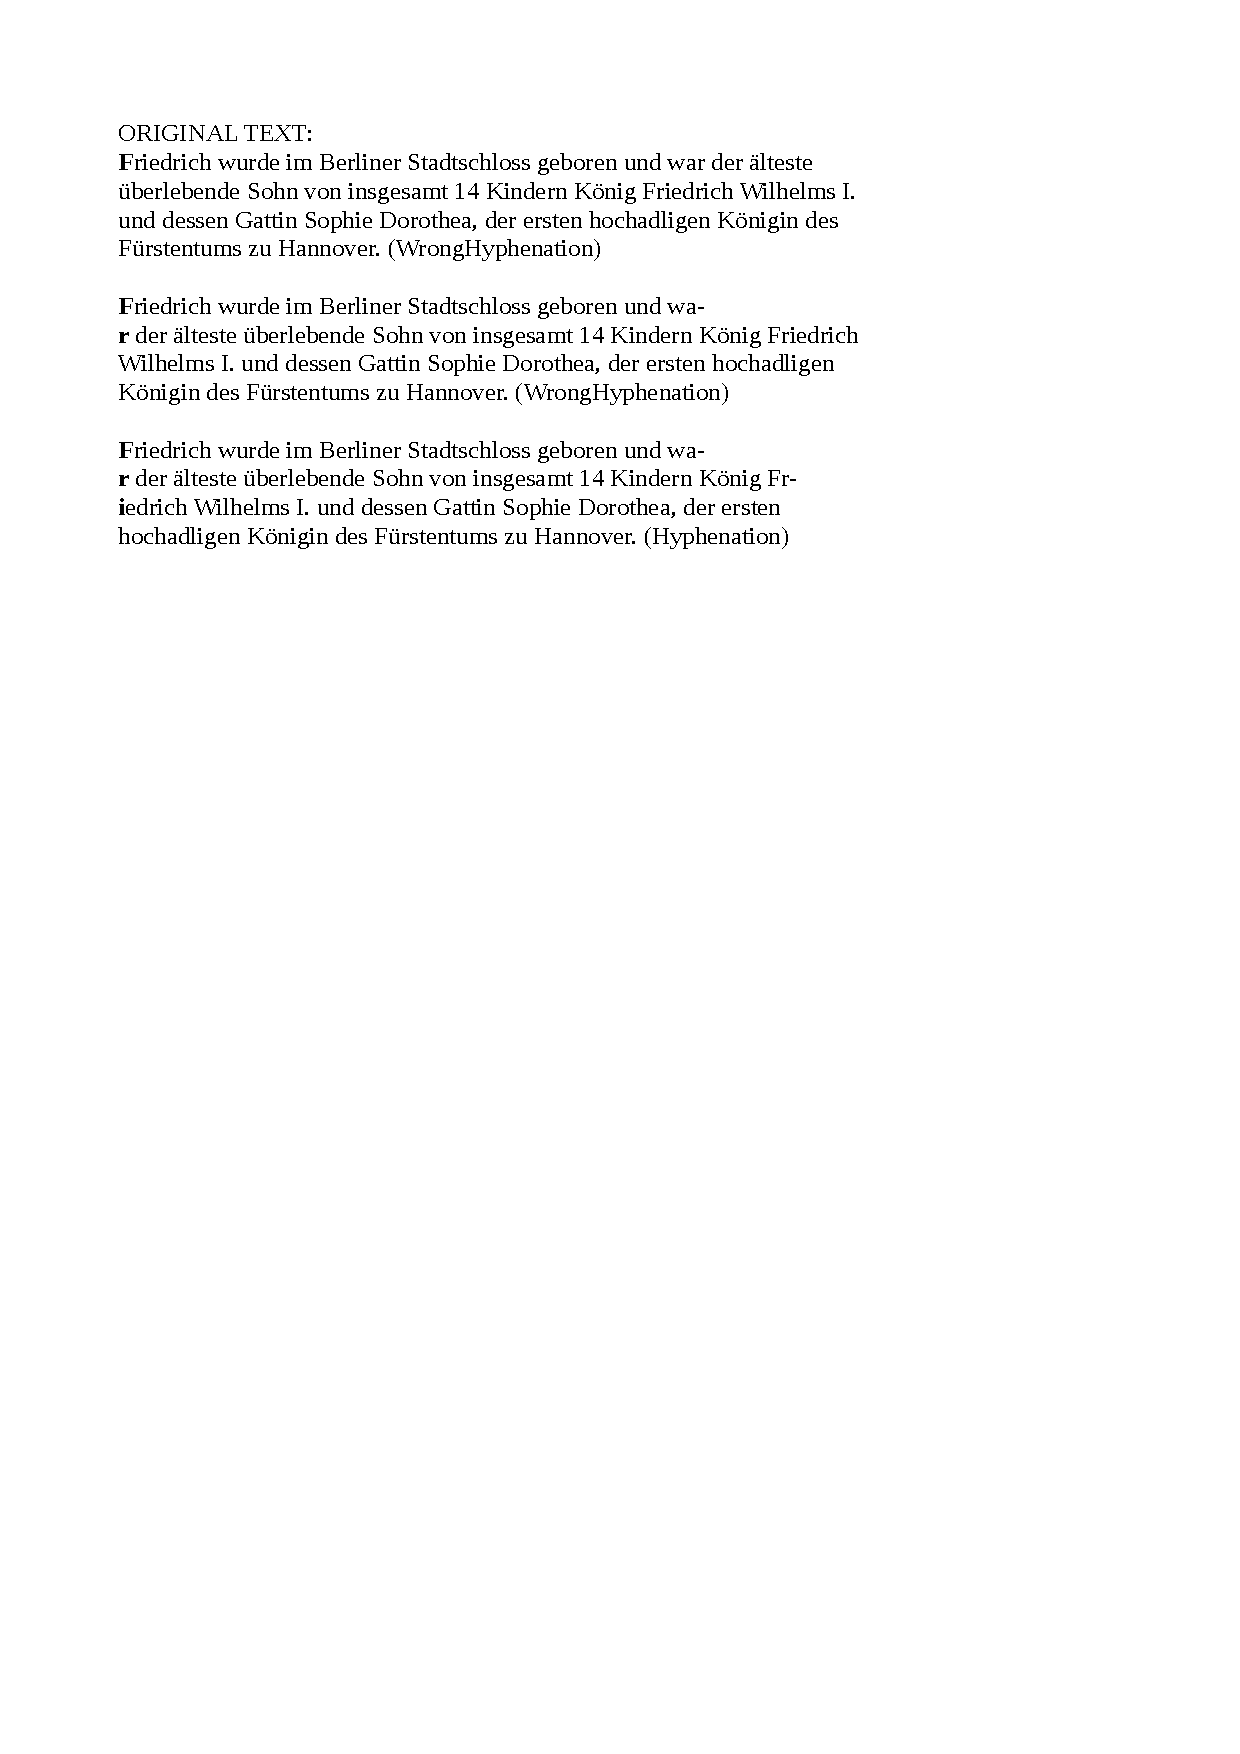
\includegraphics[scale=0.7]{FritzExample.pdf}}
\end{picture}


\end{frame}


% Here starts the 2nd slide of concluding examples

\begin{frame}
\frametitle{Examples}


\begin{itemize}



\item  1 min 22 sec, 17517 nodes, Ops: Hyph,WrHyph,LB


\end{itemize}

\begin{picture}(300,400)
\put(-10,-165){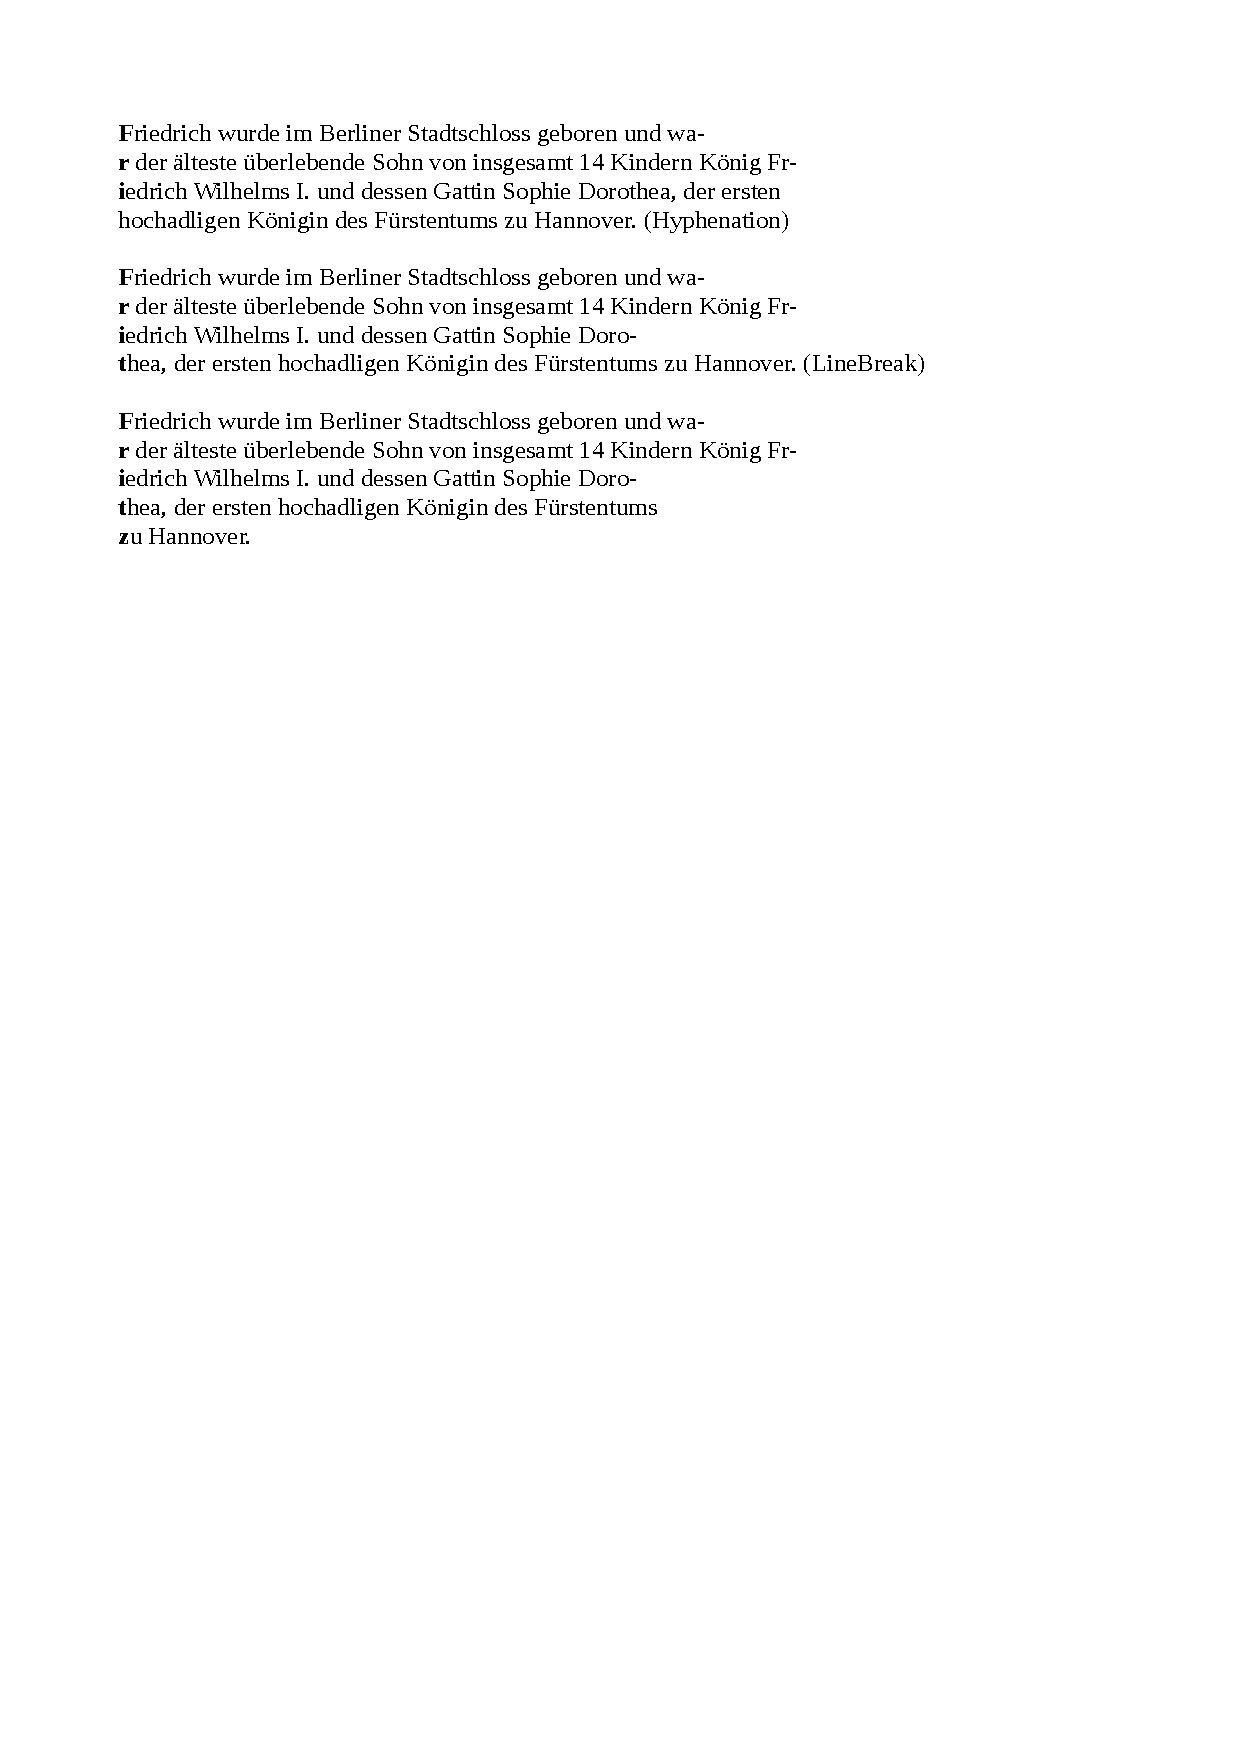
\includegraphics[scale=0.7]{FritzExample2.pdf}}
\end{picture}


\end{frame}

%********************END GENERAL EXAMPLE (all Operators included)***************************************************






%------------------------------------------------
\section{Conclusion}
%------------------------------------------------

\begin{frame}
\frametitle{Conclusion}
\begin{itemize}
\item \textbf{Operations: } Line Break, Hyphenation, Wrong Hyphenation, Synonym, Word Insertion or Deletion and Spelling.
\item \textbf{What the algorithm does:}
	\begin{itemize}
	\item Build acrostics with short words (until 6 letters) in reasonable time
	\item Build acrostics with not so good quality
	\item Success depends highly on certain conditions of the text (e.g. most of the letters of the acrostic must be in)
	\end{itemize}
\item \textbf{Difficulties:}
	\begin{itemize}
	\item The time consumed by the requests to the NGram web service
	\item The quality of the NGram database
	\item The use of NGram is sometimes too restrictive
	\item The choice of the quality of each operation is decisive in the result
	\end{itemize}
\end{itemize}
\end{frame}

%------------------------------------------------
\section{References}
%------------------------------------------------

\begin{frame}
\frametitle{References}
\scriptsize
\begin{thebibliography}{1}
\bibitem{Stein}
	Benno Stein, Matthias Hagen, and Christof Bräutigam. \emph{Generating Acrostics via Paraphrasing and Heuristic Search}. \\
	In Junichi Tsujii and Jan Hajic, editors, 25th International Conference on Computational Linguistics (COLING 14), pages 2018-2029, August 2014. Association for Computational Linguistics.
\bibitem{Spiegel}
	Spiegel Online. \emph{Griechenland und die Euro-Zone: Der fast unmögliche Rausschmiss}. \\
	http://www.spiegel.de/wirtschaft/soziales/griechenland-euro-austritt-waere-moeglich-aber-kompliziert-a-1011361.html. Am 07. Januar 2015
\bibitem{Blau}
	Hilko. \emph{Blau ist keine traurige Farbe}. \\
	https://deutschlich.wordpress.com/2013/03/12/blau-ist-keine-traurige-farbe. Am 07. Januar 2015
\bibitem{Redis}
	\emph{Redis}. http://redis.io/. Am 07. Januar 2015
\bibitem{Thesuarus}
	\emph{Synonym - OpenThesaurus - Deutscher Thesaurus}. https://www.openthesaurus.de/. Am 07. Januar 2015
\end{thebibliography}
\end{frame}
%------------------------------------------------

\begin{frame}
\Huge{\centerline{Questions?}}
\end{frame}

%----------------------------------------------------------------------------------------

\end{document}
